\documentclass{sig-alternate-05-2015}

% *** CITATION PACKAGES ***
\usepackage{cite}

% *** MATH PACKAGES ***
\usepackage{amsmath}
\usepackage{svg}
\usepackage{amsfonts}
\usepackage{bm}

% *** PDF, URL AND HYPERLINK PACKAGES ***
\usepackage{url}
\usepackage{hyperref}
\usepackage{epigraph}

% *** ALGORITHM ***
%\usepackage{algorithm}
%\usepackage{algpseudocode}
\usepackage[ruled, linesnumbered]{algorithm2e}
\renewcommand{\algorithmcfname}{ALGORITHM}
\SetAlFnt{\small}
\SetAlCapFnt{\small}
\SetAlCapNameFnt{\small}
\SetAlCapHSkip{0pt}
\IncMargin{-\parindent}

\usepackage{booktabs}
\usepackage{enumitem}
\usepackage{float}

% *** To balance reference page ***
\usepackage[keeplastbox]{flushend}

% *** Draw diagrams ***
\usepackage{tikz}
\usetikzlibrary{positioning}
\usetikzlibrary{arrows.meta}

% *** Fancy Table ***
\usepackage{multirow}

\newcommand{\paragraphb}[1]{\vspace{0.03in}\noindent{\bf #1} }
\newcommand{\paragraphe}[1]{\vspace{0.03in}\noindent{\em #1} }
\newcommand{\paragraphbe}[1]{\vspace{0.03in}\noindent{\bf \em #1} }

\newcommand{\name}{DSSnet\xspace}
\newcommand{\Name}{DSSnet\xspace}

\newtheorem{lemma}{Lemma}
\newtheorem{theorem}{Theorem}
\newdef{definition}{Definition}

% *** For commenting blocks of text ***
%\newcommand{\CUT}[1]{{}}
\begin{document}

%\begin{comment}
% DOI
%\doi{000-0-0000-0 00-0}

% ISBN
%\isbn{0000000/0000}

\CopyrightYear{2017} \setcopyright{acmcopyright}
\conferenceinfo{CS 558 Spring '17,}{March 10th, 2017, Chicago.}
\isbn{xxx-x-xxxx-xxxx-x/xx/xx}\acmPrice{\$15.00}
\doi{http://dx.doi.org/xx.xxxx/xxxxxxxxxx.xxxxxx}
%Authors, replace the red X's with your assigned DOI string.
\clubpenalty=10000
\widowpenalty = 10000
%\end{comment}

%
% --- Author Metadata here ---
%\conferenceinfo{WOODSTOCK}{'97 El Paso, Texas USA}
%\CopyrightYear{2007} % Allows default copyright year (20XX) to be over-ridden - IF NEED BE.
%\crdata{0-12345-67-8/90/01}  % Allows default copyright data (0-89791-88-6/97/05) to be over-ridden - IF NEED BE.
% --- End of Author Metadata ---

\title{A Comparative Study of Deep Learning Approaches in Off-Line Network Intrusion Detection}
\subtitle{[Project Report]
\titlenote{The codebase for our project is available on https://github.com/littlepretty/NetLearner}}

%
% You need the command \numberofauthors to handle the 'placement
% and alignment' of the authors beneath the title.
%
% For aesthetic reasons, we recommend 'three authors at a time'
% i.e. three 'name/affiliation blocks' be placed beneath the title.
%
% NOTE: You are NOT restricted in how many 'rows' of
% "name/affiliations" may appear. We just ask that you restrict
% the number of 'columns' to three.
%
% Because of the available 'opening page real-estate'
% we ask you to refrain from putting more than six authors
% (two rows with three columns) beneath the article title.
% More than six makes the first-page appear very cluttered indeed.
%
% Use the \alignauthor commands to handle the names
% and affiliations for an 'aesthetic maximum' of six authors.
% Add names, affiliations, addresses for
% the seventh etc. author(s) as the argument for the
% \additionalauthors command.
% These 'additional authors' will be output/set for you
% without further effort on your part as the last section in
% the body of your article BEFORE References or any Appendices.


%\begin{comment}
\numberofauthors{2} %  in this sample file, there are a *total*
% of EIGHT authors. SIX appear on the 'first-page' (for formatting
% reasons) and the remaining two appear in the \additionalauthors section.
%

\author{
% You can go ahead and credit any number of authors here,
% e.g. one 'row of three' or two rows (consisting of one row of three
% and a second row of one, two or three).
%
% The command \alignauthor (no curly braces needed) should
% precede each author name, affiliation/snail-mail address and
% e-mail address. Additionally, tag each line of
% affiliation/address with \affaddr, and tag the
% e-mail address with \email.
%
% 1st. author
\alignauthor
Jiaqi Yan\\
      \affaddr{Illinois Institute of Technology}\\
       \affaddr{10 West 31st Street}\\
       \affaddr{Chicago, Illinois, 60616 }\\
       \email{jyan31@hawk.iit.edu}
% 2nd. author
\alignauthor
Dong Jin\\
       \affaddr{Illinois Institute of Technology}\\
       \affaddr{10 West 31st Street}\\
       \affaddr{Chicago, Illinois, 60616 }\\
       \email{dong.jin@iit.edu}
% 3rd. author
%\alignauthor
%Dong Jin\\
       %\affaddr{Illinois Institute of Technology}\\
       %\affaddr{10 West 31st Street}\\
       %\affaddr{Chicago, Illinois, 60616 }\\
       %\email{dong.jin@iit.edu}
%\and  % use '\and' if you need 'another row' of author names
%% 4th. author
%\alignauthor Lawrence P. Leipuner\\
%       \affaddr{Brookhaven Laboratories}\\
%       \affaddr{Brookhaven National Lab}\\
%       \affaddr{P.O. Box 5000}\\
%       \email{lleipuner@researchlabs.org}
%% 5th. author
%\alignauthor Sean Fogarty\\
%       \affaddr{NASA Ames Research Center}\\
%       \affaddr{Moffett Field}\\
%       \affaddr{California 94035}\\
%       \email{fogartys@amesres.org}
%% 6th. author
%\alignauthor Charles Palmer\\
%       \affaddr{Palmer Research Laboratories}\\
%       \affaddr{8600 Datapoint Drive}\\
%       \affaddr{San Antonio, Texas 78229}\\
%       \email{cpalmer@prl.com}
}

%\end{comment}

\maketitle
\begin{abstract}
Recently, a handful of novel deep neural networks have achieved unprecedentedly
good performance on image classification, natural language processing,
speech recognition and many other artificial intelligence related research fields.
In this project we investigate the possibility of applying the cutting edge
deep learning techniques to the classic network intrusion detection system.
We specifically look at a well-known public network intrusion dataset and
compare the performance of several popular deep neural network architectures
on this particular NSL-KDD dataset.
At this report, we
\begin{itemize}
        \item describe how we processing the NSL-KDD dataset so that
        it can be fed to deep neural networks;
        \item briefly introduce each deep neural network considered in this project;
        {\color{red}\item implement and train multi-layer percetron, restricted Boltzmann machine,
                sparse autoencoder and denoising autoencoder in TensorFlow;
        \item evaluate the classification performance in terms of accuracy, precision,
                recall as well as F1-Score}\footnote{Contents in red are new progress from mid-term.}
\end{itemize}
The listed achievements above will serve as the basis in conducting
a comparative study of deep learning approaches in network intrusion detection.
\end{abstract}

%
%  Use this command to print the description
%
%\printccsdesc

% We no longer use \terms command
%\terms{Theory}

\keywords{Network Intrusion Detection System; Deep Learning}

\section{Introduction}

Network intrusion detection system is device or software application that monitors a network
for malicious activities or policy violations.
By intercepting and analysing the incoming or outgoing traffics through the network,
it raises alarm if intrusion or attack is observed.
There are two general approaches to detect intrusions.
In signature based intrusion detection, e.g. SNORT~\cite{Snort}, rules for specific attacks
are pre-installed in the system.
It raises alarm when traffic match the signature of known attacks.
The major drawbacks of signature matching approach is that
it is only effective for previously detected attacks that have an identifiable signature.
As a result, signature database needs to be manually updated whenever a new type of attack
is discovered, with significant effort, by the network administrator.
Anomaly detection based approach overcomes the these limitations by adopting a certain
type of machine learning technique to model the trustworthy network activities.
Traffics that significantly deviates from the built model are treated as malicious.
This idea have been shown to be able to detect unknown or novel attacks~\cite{NSL-KDD, STL-NIDS}.




More background information will be available in the final report,
for example, introducing back-propagation~\cite{Backpropagation}.

\section{Data Processing}


\section{Deep Neural Networks}
In this section, we give a brief review of the deep learning architectures that we used
in network intrusion detection problem.

\subsection{Multilayer Perceptron}
Multilayer perceptron (MLP) is the simplest deep learning classifier in terms of
design of the architecture.
It is a fully connected feed-forward neural network, as shown in Figure~\ref{Fig:MLPArchitecture}.
By introducing non-linear neural units (perceptron), it can distinguish data that are
not linearly separable.
However, the non-linearity also make it very hard to train a deep MLP,
even if people have proposed the efficient back-propagation learning algorithm~\cite{Backpropagation}.
Recently it revived due to various new training techniques designed by deep learning community,
including Stochastic Gradient Descent (SGD),
batch normalization~\cite{BatchNorm} and Dropout~\cite{Dropout}.
Expect for the number of neurons in each layer and number of layers,
MPL can also be tuned with different activation functions, or neural types.
The most popular two, which are used in this project, are logistic function
and rectifier linear unit.
Logistic function is written as
\begin{align}
        f(x) &= \frac{1}{1 + e^{-x}}
\end{align}
It has a very useful property when we applying backpropagation:
\begin{align}
        f'(x) &= f(x) (1-f(x))
\end{align}
Recently, most deep neural networks adopt rectifier neural unit and achieved very good performance~\cite{DeepLearning}.
Rectifier linear unit is defined as
\begin{align}
        f(x) &= \max(0, x)
\end{align}
Let $\mathbf{a}^{(l)}$ be the activation of layer $l$,
$\mathbf{W}^{(l)}$ and $\mathbf{b}^{(l)}$ be layer $l$'s parameter.
With activation function defined, we have the following recursive formula that describes
the feed-forward step of the perceptron network.
\begin{align}
        \mathbf{z}^{(l+1)} &= \mathbf{W}^{(l)} \mathbf{a}^{(l)} + \mathbf{b}^{(l)} \\
        \mathbf{a}^{(l+1)} &= f(\mathbf{z}^{(l+1)})
\end{align}

\begin{figure}[h]
\centering
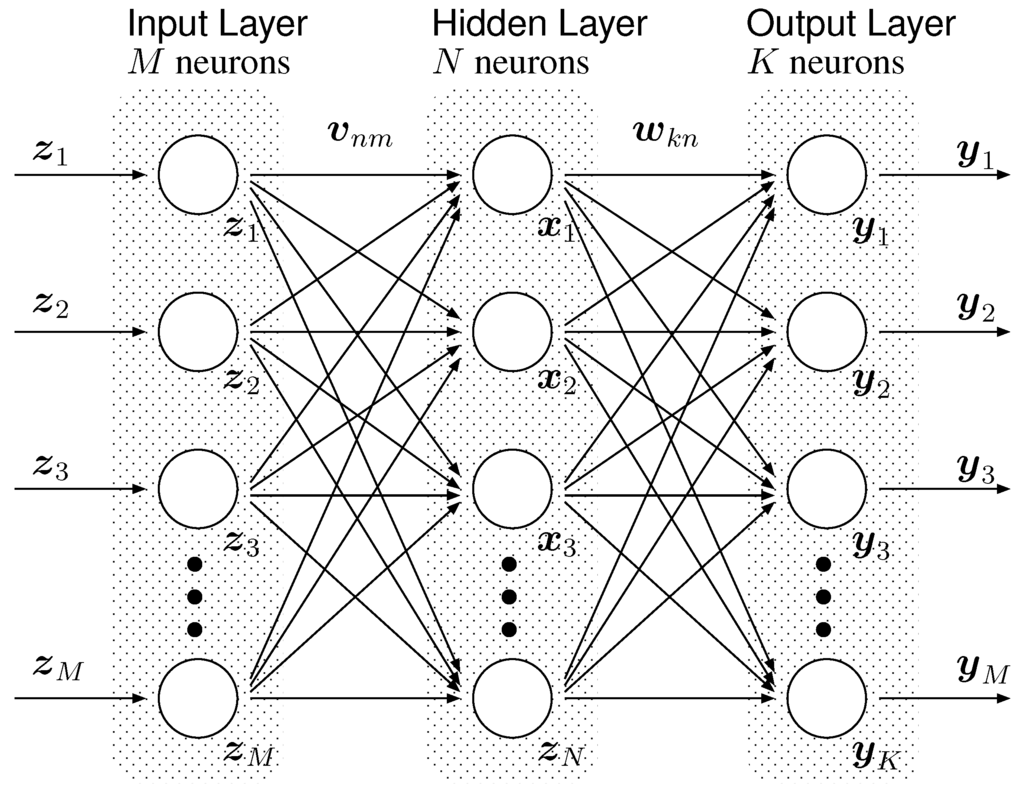
\includegraphics[width=0.45\textwidth]{figures/multilayer_perceptron.png}
\caption{A perceptron neural network with 1 hidden layer.
        Figure courtesy of Teijiro Isokawa, Haruhiko Nishimura and Nobuyuki Matsui.}
\label{Fig:MLPArchitecture}
\end{figure}

\subsection{Generative Models}
The amount of network traffic data is enormously large, usually in the order of terabytes
per day in a large monitored network.
This available big data makes deep learning techniques a promisingly better solution
to traffic classification.
In practice, however, the amount of data is impossible for a human security analyst to review,
e.g., to find patterns and label anomalies.
Generative model which can be trained unsupervisedly comes to rescue in that
\begin{itemize}
\item It utilizes the large amount of unlabeled data to learning useful and hierarchical features;
\item It is actually a way to initialize the weights in a deep neural network, which can be
        further fine-tuned to be a high performance classifier.
\end{itemize}
In this project we propose to try two generative models: restricted Boltzmann machine and autoencoders.

\subsubsection{Restricted Boltzmann Machine}
Restricted Boltzmann machine (RBM) consists of a layer of hidden units (H) and a layer of visible units (V).
Here, ``restricted" means that connections are just between hidden and visible layer,
but not within hidden layers or visible layers.
This make training RBM faster than Boltzmann machine and feasible for stacking together
to form deep architecture.
After learning the first layer RBM, the activity vector of the hidden units can be used
as ``data" for training the second layer RBM
and this process can be repeated to learn as many hidden layers as desired.
As data passing through the RBMs, we can obtain the highest level features 
which are typically fed into a classifier.
The entire deep network (RBMs plus the classifier) can be fine-tuned to
improve the classification performance.

\begin{align}
        E(\mathbf{v, h}) &= -\sum_i b_i v_i - \sum_j b_j h_j - \sum_{i, j} v_i h_j w_{ij} \\
        \Delta w_{ij} &= \epsilon (<v_i h_j>_{data} - <v_i h_j>_{reconstruction}) \\
        Prob(h_j = 1) &= sigmoid(b_j + \sum_i{v_i w_{ij}}) \\
\end{align}



\subsubsection{Autoencoders}
An autoencoder neural network is an unsupervised model with typically one hidden layer that
tries to set the output layer to be equal to the input.
As shown in Figure~\ref{Fig:AEArchitecture}, we want the network to
learn a function $h_{W, b}(x) \approx x$.
However, to prevent the network from learning the meaningless identify function,
we need to place extra constraints on the network, which introduces many different
flavors of autoencoders.
In this project we consider two most popular type of autoencoders, sparse autoencoder and
denoise autoencoder.

The \textbf{denoising autoencoder} algorithm is proposed by~\cite{DenoiseAE} and illustrated in
Figure~\ref{Fig:dAEAlgorithm}.
To prevent learning identify function, an example $\mathbf{x}$ is first corrupted, either by
adding Gaussian noise or by random masking a fraction of items in $\mathbf{x}$ to zero.
The autoencoder then maps corrupted $\mathbf{\tilde{x}}$ to a hidden representation $\mathbf{y} = sigmoid(\mathbf{W}\tilde{\mathbf{x}} + \mathbf{b})$.
From $\mathbf{y}$ we reconstruct a $\mathbf{z}=g_\theta'(\mathbf{y})$.
The training needs to learning the parameters $\theta$ and $\theta'$ so that average reconstruction error is minimized over training set.
For binary input $\mathbf{x}$, usually cross entropy is adopted as $L_H(\mathbf{x}, \mathbf{z})$;
while mean squared error is used for real-valued $\mathbf{x}$.

\begin{figure}[h]
\centering
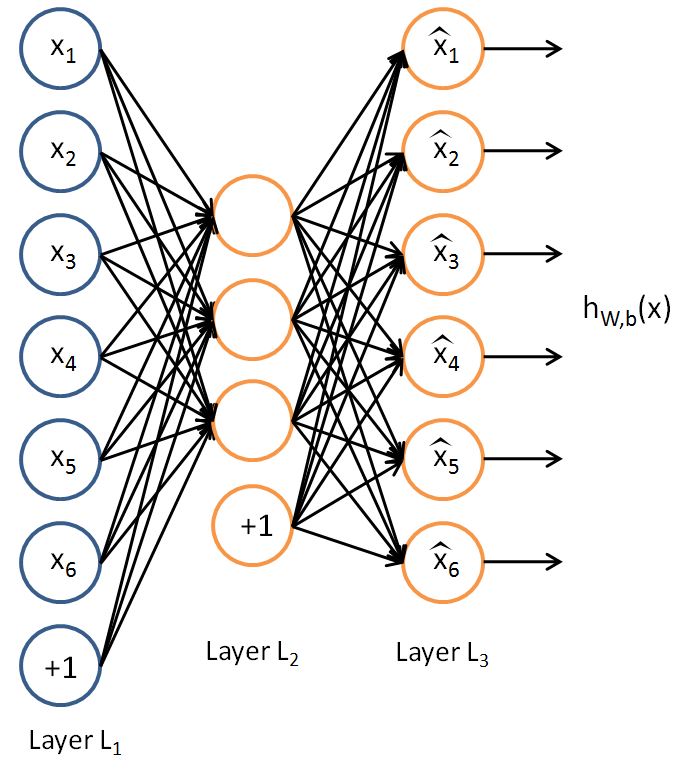
\includegraphics[width=0.45\textwidth]{figures/autoencoder.png}
\caption{General Architecture of Autoencoders.
        Figure courtesy of~\cite{UFLDLAutoencoder}.}
\label{Fig:AEArchitecture}
\end{figure}

\begin{figure}[h]
\centering
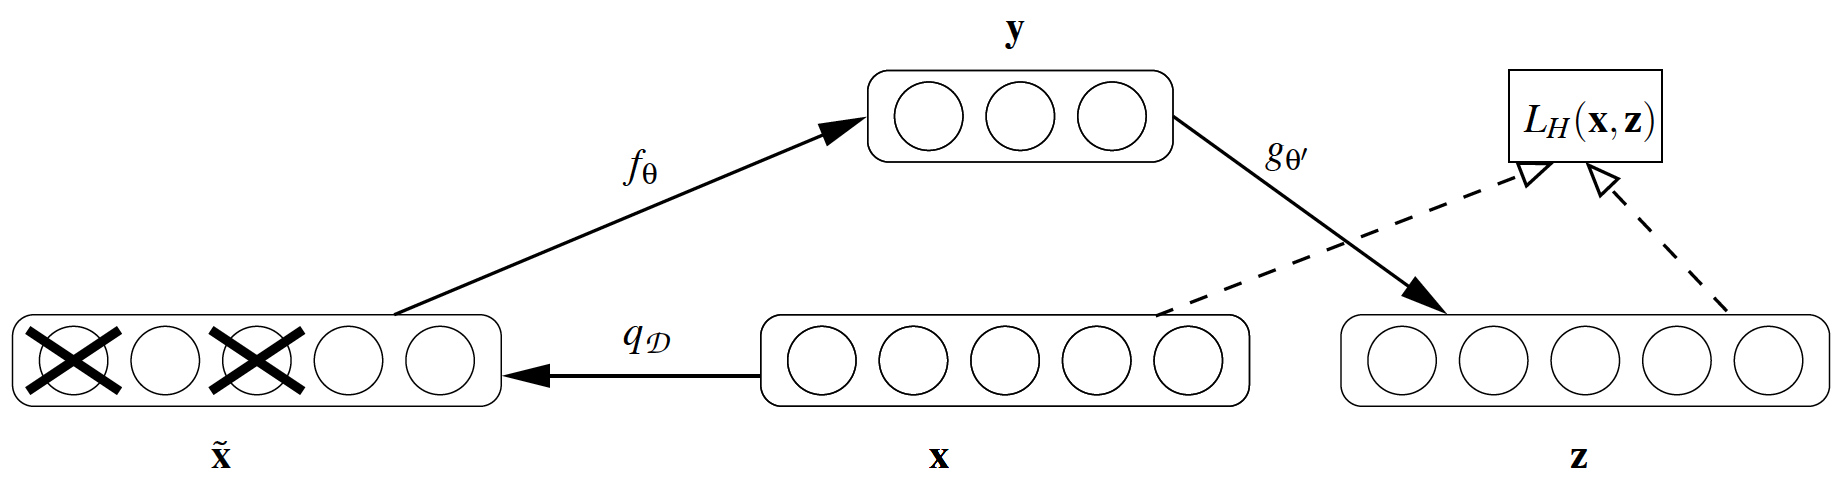
\includegraphics[width=0.45\textwidth]{figures/denoiseautoencoder.png}
        \caption{The denoising autoencoder algorithm.
        Input example $\mathbf{x}$ is randomly corrupted via $q_\mathcal{D}$ and then
        is mapped via encoder $f_\theta$ to $\mathbf{y}$.
        The decoder $g_\theta'$ attempts to reconstruct $\mathbf{x}$ and produces $\mathbf{z}$.
        Reconstruction error is measured by loss $L_H(\mathbf{x}, \mathbf{z})$, to be minimized
        during the training phase.}
\label{Fig:dAEAlgorithm}
\end{figure}

The \textbf{sparse autoencoder} works by placing a sparsity constraint on the hidden units~\cite{SparseAE}.
First, we make the autoencoder's hidden layer size to be over-complete,
that is of larger size comparing to the dimension of the input.
Let's denote the activation of hidden unit $j$ of layer 2 in Figure~\ref{Fig:AEArchitecture}
to be $a^2_j(\mathbf{x})$ given input example $\mathbf{x}$.
With that, we can define the average activation of hidden unit $j$ over the $m$-size
training set
\begin{align}
        \hat{\rho}_j = \frac{1}{m} \sum_{i=1}^{m} a^2_j(\mathbf{x})
\end{align}
The sparsity constraint is enforcing, $\forall$ hidden unit $j$,
\begin{align}
        \hat{\rho}_j = \rho
\end{align}
where $\rho$ is a sparsity parameter that approximates zero (say 0.05).
This constraint can be vectorized over the hidden layer, say of size $n_2$,
with the KL divergence based penalty term
\begin{align}
        \sum_j^{n_2} KL(\rho || \hat{\rho}_j)
        = \sum_j^{n_2} [\rho \log \frac{\rho}{\hat{\rho}_j} + (1 - \rho) \log \frac{1-\rho}{1-\hat{\rho}_j} ]
\end{align}
The sparsity penalty term is integrated into the cost function by adding another hyperparameter $\beta$
\begin{align}
        L(W, b) = \frac{1}{2}||h_{W,b}(\mathbf{x}) - \mathbf{x}||^2 + \beta \sum_j^{n_2} KL(\rho || \hat{\rho}_j)
\end{align}

Denoise autoencoder and sparse autoencoder, surprisingly, have different application domains.
Vincent et al.~\cite{DenoiseAE} have shown that stacked denoise autoencoder can be used to
initialize a deep neural network's weight parameter,
achieving similar and sometimes better performance than stacked RBM.
They also show that training stacked denoise autoencoder with MNIST dataset, it is able
to resynthesize a variety of similarly good quality digits.
Raina et al.~\cite{SparseAE} have compared sparse encoding with principle component analysis
(PCA) and argue that transfer raw features with a well unsupervisely trained
sparse audoencoder can be beneficial to supervised learning algorithm,
for example support vector machine (SVM).

\section{Implementation}

\subsection{TensorFlow 101}
TensorFlow~\cite{TensorFlow} is an open-source software library for machine learning developed by the Google Brain Team.
Multidimensional data arrays are presented as tensor data structure in TensorFlow.
The user of the library can constructs a graph to implement any general machine learning algorithm.
Nodes in the graph represent mathematical operations between tensors,
such as add, multiply, softmax and dropout.
Graph edges represent the flow of tensors between nodes.
The computation graph based architecture allow researchers to run or train neural networks
on one or more CPUs or GPUs with unified API.

For general classification task, input $X$ and label $Y$ are defined as \textbf{placeholder}s
and feed into the computation graph at running time using a dictionary.
The graph of a typical deep learning model have three parts.
The \textbf{inference} graph should be built so that output predictions could be returned as tensor.
For example, in the multilayer perceptron case, inference graph contains all iterative
computation~\ref{Equ:MLPFeedForward1}-\ref{Equ:MLPFeedForward2} in the feed-forwarding steps.
The \textbf{loss} graph should compute the loss function defined by particular models.
Usually it is either cross-entropy or mean-squared error averaged across the batch data.
The loss graph will be optimized, usually minimized, by the \textbf{train} part.
This optimization can be conducted by various optimizing algorithms, such as gradient descent,
Momentum, RMSProp.
After sufficient steps of batch training, we can evaluate the trained model with inference
graph and compare the predictions with the test dataset labels.
TensorFlow also provides various useful utilities for training models and running experiments.
Using a Saver, we are able to checkpoint the training process used to later restore a model for
further training or evaluation.
User can also use Summary nodes to log the snapshot of interest variables, which can be
automatically visualized by TensorBoard.

\subsection{NetLearner}
We provide a Python library NetLearner that wraps up several deep learning models on the basis of TensorFlow.
NetLearner modularizes multilayer perceptron, restricted Boltzmann machine, sparse autoencoder
and masking-noise autoencoder, all of which are used to perform the 5-class classification
on the NSL-KDD dataset.

For the multiple layer perceptron, we tried a 4-hidden-layer network with
very wide size in each layer, several hundreds for each layer.
The accuracy on training set is very exiting, usually more than 96\%.
However, its performance on test dataset is not satisfactory at all.
Instead we found out that a single hidden layer with only forty neurons has terrific accuracy.
It is trained with stochastic gradient descent (SGD) for 20 epochs and batch size 100.
During the training, learning rate decays from 0.1 exponentially with the base of 0.32.
We did not include regularization in the model, but did apply dropout of keep probability 0.8.
We denote this approach as MLP and show its detailed results in the later section.

We build a RBM with 200-hidden units to perform unsupervised feature learning first on the dataset.
The learned features are then fed into a simple softmax regression classifier.
We trained the RBM using CD1 (contrastive divergence using one full step to get the negative data),
with batch size 10 for 40 epochs.
The learning rate is initialized at 0.01 and decay exponentially with the base of 0.64.
We denote this combination of RBM and softmax regression as RBM in the later section.

We also implemented the self-taught learning architecture proposed in~\cite{STL-NIDS, SparseAE},
adopting sparse autoencoder as the unsuperviesed feature learner.
The learnt features will then be used for classification by a Softmax regression classifier.
We contact the author of~\cite{STL-NIDS} so that we can reproduce their implementation
with the same hyper-parameters.
For example, the hidden layer size of the sparse autoencoder is 64;
the sparsity value $\rho$ is 0.25.
Different from~\cite{STL-NIDS}, we found that using regularization in
neither autoencoder nor softmax regression is helpful.
So we didn't include regularization term in the both autoencoder and softmax cost function.
The autoencoder is trained with SGD for 1000 epochs and batch size 5000.
Different from MLP, we used Adam optimizer during the training.
The learning rate starts at 0.01 and decay exponentially with base of 0.6.
We denote this approach as SAE and report its performance in the later section.

As a variation to the sparse autoencoder based self-taught learning arhictecture,
we explore what will the performance be if we replace sparse autoencoder with denosing autoencoder.
We simple use dropout to emulate the masking noise to build masking noise autoencoder,
in which input is randomly masked out with keep probability of 0.4.
The size of the denoising autoencoder is 100.
The autoencoder is trained with SGD for 1000 epochs and batch size 5000.
We trained denoising autoencoder in the same way as we trained sparse autoencoder.
The result of this approach is labeled as DAE in the later section.

One thing to notice is that we use the same seed to randomly initialized the weights and biases
of the softmax regression classifier such that the learnt features from RBM, sparse autoencoder and
denoising autoencoder are comparable.
For the same reason, all the softmax regression classifiers used by RBM, sparse autoencoder and
denoising autoencoder are trained with Adam optimizer of batch size 100 for 100 epochs,
with exponentially decay learning rate starting at 0.01, with dropout of keep probability 0.8.

\section{Experiment Results}

\subsection{Evaluation Metrics}
We evaluate the classification performance of our proposed deep learning approaches
with the following metrics.
\begin{itemize}
    \item \textbf{Accuracy} is the percentage of correctly classified connections
        over the total number of connections in the dataset:
        \begin{align}
            A = \frac{\text{Correct Predictions}}{\text{Number of Records}}
        \end{align} 
        Accuracy is not suitable for evaluating biased dataset where the number
        of records of some class is extremely larger than the number of
        records of another class.
        In NSL-KDD dataset, the number of available U2R records (67)
        is in two degrees of magnitude less than the other classes of traffic (9711, 7458, 2887, 2121 respectively).
        Therefore we also consider the following metrics.
    \item \textbf{Precision} is the percentage of the correctly classified positives over
        the total number of positives predicted by the classifier:
                \begin{align}
                    P = \frac{\text{True Positives}}{\text{True Positives} + \text{False Positives}}
                \end{align}
            \item \textbf{Recall} is the percentage of the correctly classified positives over
                the total number of relevant elements:
                \begin{align}
                    R = \frac{\text{True Positives}}{\text{True Positives} + \text{False Negatives}}
                \end{align}
            \item \textbf{F1-Score} represents a balance between precision and recall and is calculated
                as their harmonic mean:
                \begin{align}
                    F = \frac{2PR}{P + R}
                \end{align}
\end{itemize}
Besides, we also provide the confusion matrix of the classification results when applying
different approaches on the test dataset.
In our confusion matrix table, the row represents the instance in an actual class,
while the column represents the instance in a predicted class.
This table is useful for visualizing how the adopted approach is confusing one class with
other classes.

\subsection{Performance of Deep Learning Approaches}

\begin{figure}[h]
    \centering
    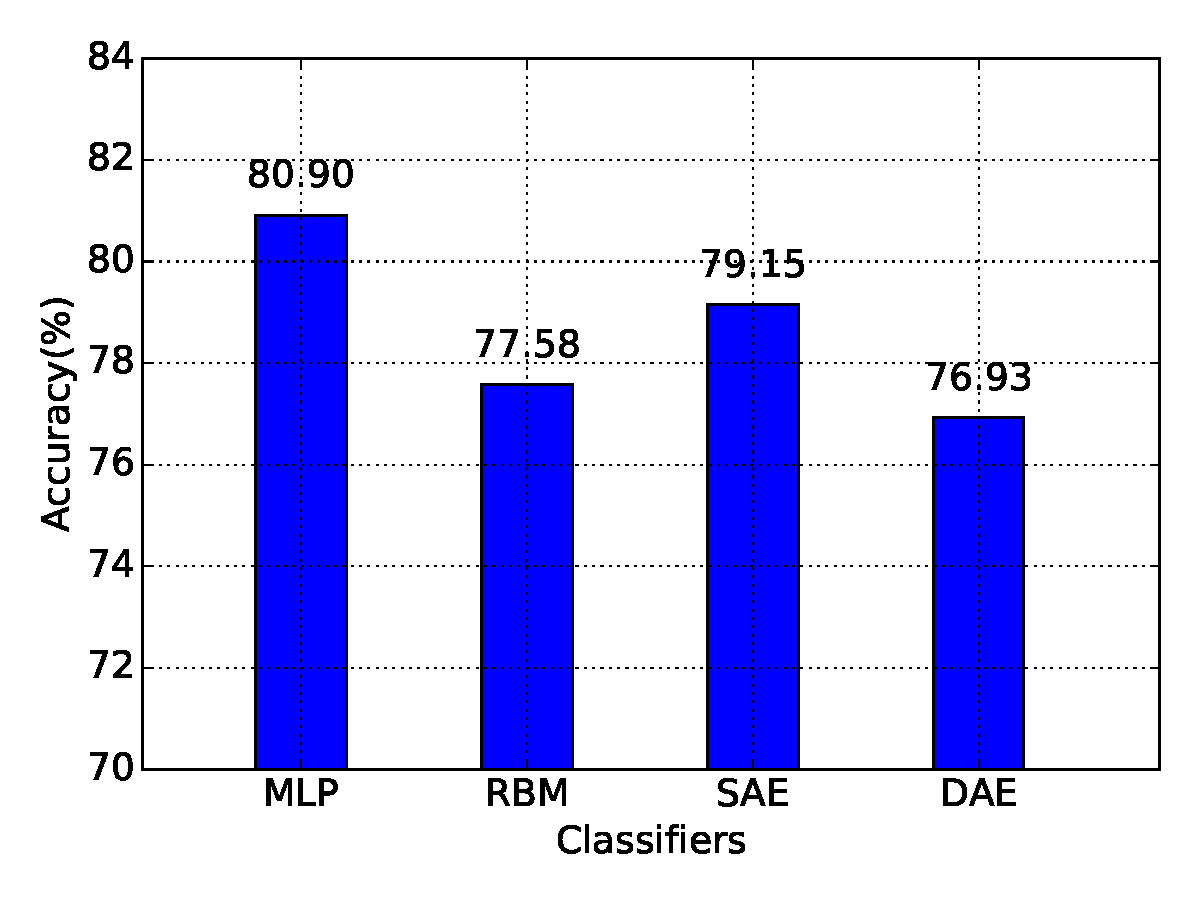
\includegraphics[width=0.48\textwidth]{figures/comp_accuracy.pdf}
    \caption{Classification Accuracy of Proposed Approaches}
    \label{Fig:CompAccuracy}
\end{figure}

\begin{table}[t]
    \caption{Confusion Matrix of MLP on Test Dataset}
    \centering
    \begin{tabular}{cc|rrrrr}
        \hline
        &  & \multicolumn{5}{c}{Prediction} \\
                        &        & Normal & Probe & DoS & U2R & R2L\\
        \hline
        \hline
        \multirow{5}{*}{Actual} & Normal & 8788 &  316 &  473 &  67 &   67 \\
                                &  Probe &   13 & 2111 &  235 &  13 &   53 \\
                                &  DoS   &  798 &  157 & 6258 & 420 &    4 \\
                                &  U2R   &  337 &    4 &    1 &  50 &    4 \\
                                &  R2L   &  869 &  126 &    3 & 491 &  887 \\
        \hline
        \multicolumn{2}{c|}{Precision(\%)}   & 96.10& 77.65& 79.90&  9.09& 31.36\\
        \multicolumn{2}{c|}{Wtd. Avg.(\%)}   & \multicolumn{5}{r}{71.88}\\
        \hline
        \multicolumn{2}{c|}{Recall(\%)}      & 74.92& 80.85& 95.19& 10.06& 75.10 \\
        \multicolumn{2}{c|}{Wtd. Avg.(\%)}   & \multicolumn{5}{r}{68.66}\\
        \hline
        \multicolumn{2}{c|}{F1-Score(\%)}    & 84.20& 79.22& 86.88&  9.55& 44.24 \\
        \multicolumn{2}{c|}{Wtd. Avg.(\%)}   & \multicolumn{5}{r}{68.73}\\
        \hline
    \end{tabular}
\end{table}


\begin{table}[t]
    \caption{Confusion Matrix of RBM on Test Dataset}
    \centering
    \begin{tabular}{cc|rrrrr}
        \hline
        &  & \multicolumn{5}{c}{Prediction} \\
                        &        & Normal & Probe & DoS & U2R & R2L\\
        \hline
        \hline
        \multirow{5}{*}{Actual} & Normal & 8788 &  316 &  473 &  67 &   67 \\
                                & Probe  &   13 & 2111 &  235 &  13 &   53 \\
                                & DoS    &  798 &  157 & 6258 & 420 &    4 \\
                                & U2R    &  337 &    4 &    1 &  50 &    4 \\
                                & R2L    &  869 &  126 &    3 & 491 &  887 \\
        \hline
        \multicolumn{2}{c|}{Precision(\%)}   & 81.34& 77.78& 89.78& 4.80& 87.39\\
        \multicolumn{2}{c|}{Wtd. Avg.(\%)}   & \multicolumn{5}{r}{71.04}\\
        \hline
        \multicolumn{2}{c|}{Recall(\%)}      & 90.50& 87.05& 81.95& 12.63 &37.33\\
        \multicolumn{2}{c|}{Wtd. Avg.(\%)}   & \multicolumn{5}{r}{73.65}\\
        \hline
        \multicolumn{2}{c|}{F1-Score(\%)}    & 85.67& 82.16& 85.69 &6.96 &52.31\\
        \multicolumn{2}{c|}{Wtd. Avg.(\%)}   & \multicolumn{5}{r}{70.84}\\
        \hline

    \end{tabular}
\end{table}

\begin{table}[t]
    \caption{Confusion Matrix of SAE on Test Dataset}
    \centering
    \begin{tabular}{cc|rrrrr}
        \hline
        &  & \multicolumn{5}{c}{Prediction} \\
                        &        & Normal & Probe & DoS & U2R  & R2L\\
        \hline
        \hline
        \multirow{5}{*}{Actual}  & Normal & 8864 &  696 &   92 &   11 &   48 \\
                                 & Probe  &  179 & 2001 &  164 &    2 &   79 \\
                                 & DoS    & 1542 &   39 & 6054 &    0 &    1 \\
                                 & U2R    &  357 &    1 &    1 &   30 &    7 \\
                                 & R2L    & 1444 &    6 &    5 &   26 &  895 \\
        \hline
        \multicolumn{2}{c|}{Precision(\%)}    & 71.56& 72.95& 95.85& 43.48& 86.89\\
        \multicolumn{2}{c|}{Wtd. Avg.(\%)}    & \multicolumn{5}{r}{81.06}\\
        \hline
        \multicolumn{2}{c|}{Recall(\%)}       & 91.28& 82.52& 79.28&  7.58& 37.67\\
        \multicolumn{2}{c|}{Wtd. Avg.(\%)}    & \multicolumn{5}{r}{79.15}\\
        \hline
        \multicolumn{2}{c|}{F1-Score(\%)}     & 80.23& 77.44& 86.78& 12.90& 52.55\\
        \multicolumn{2}{c|}{Wtd. Avg.(\%)}    & \multicolumn{5}{r}{\color{red}78.05}\\
        \hline
    \end{tabular}
\end{table}


\begin{table}[t]
    \caption{Confusion Matrix of DAE on Test Dataset}
    \centering
    \begin{tabular}{cc|rrrrr}
        \hline
        &  & \multicolumn{5}{c}{Prediction} \\
                        &        & Normal & Probe & DoS & U2R & R2L\\
        \hline
        \hline
        \multirow{5}{*}{Actual} & Normal & 9249 &  319 &   85 &  10 &  48 \\
                                & Probe  & 576  & 1504 &  226 &   2 & 117 \\
                                & DoS    & 1842 &  128 & 5665 &   0 &   1 \\
                                & U2R    & 353  &    1 &    0 &  38 &   4 \\
                                & R2L    & 1469 &    3 &    1 &  17 & 886 \\
        \hline
        \multicolumn{2}{c|}{Precision(\%)} & 68.57& 76.93& 94.78& 56.72& 83.90\\
        \multicolumn{2}{c|}{Wtd. Avg.(\%)} & \multicolumn{5}{r}{79.75}\\
        \hline
        \multicolumn{2}{c|}{Recall(\%)}    & 95.24& 62.02& 74.19&  9.60& 37.29\\
        \multicolumn{2}{c|}{Wtd. Avg.(\%)} & \multicolumn{5}{r}{76.93}\\
        \hline
        \multicolumn{2}{c|}{F1-Score(\%)}  & 79.73& 68.68& 83.23& 16.41& 51.63\\
        \multicolumn{2}{c|}{Wtd. Avg.(\%)} & \multicolumn{5}{r}{75.65}\\
        \hline
    \end{tabular}
\end{table}


\section{Conclusion}
In this project we conducted a comparative study on the deep learning approaches
for the network intrusion detection problem.
We take the off-line network intrusion detection dataset NSL-KDD for evaluation.
In this paper, multi-layer perceptron, restricted boltzmann machine, sparse autoencoder
and denoising autoencoder are briefly described.
The main contribution lies on the comparable evaluation of these introduced approaches.
From our experiment results, we conclude that for the NSL-KDD test dataset,
multi-layer perceptron has comparably best performance since both its accuracy and F1-Score
are outstanding.



%
% The following two commands are all you need in the
% initial runs of your .tex file to
% produce the bibliography for the citations in your paper.
\bibliographystyle{abbrv}
\bibliography{sigproc}  % sigproc.bib is the name of the Bibliography in this case
% You must have a proper ".bib" file
%  and remember to run:
% latex bibtex latex latex
% to resolve all references
%
% ACM needs 'a single self-contained file'!
%

%\nocite{*}
%\balancecolumns % GM June 2007
% That's all folks!
\end{document}
